\chapter{Graph-Datenbanken im praktischen Einsatz: OLTP}
\section{PostgresSQL: OLTP}
\subsection{Ausgewählte Use Cases}
Die Aufgabe ist es 5 Graphen mit Hilfe der Breitensuche zu traversieren. Hierfür soll keine Graphdatenbank verwendet werden, sondern eine objektrelationale Datenbank.
Die Vermutung ist, dass das Traversieren eines Graphen mit Hilfe einer objektrelationalen Datenbank ähnlich schnell ist, wie das Traversieren mit Hilfe einer Graphdatenbank.
Für die Graphtraversierung sind 5 Methoden vorgesehen:
\begin{itemize}
    \item Graphtraversierung mit Hilfe von Standard SQL (SELECT WITH UNION)
    \item Graphtraversierung mit Hilfe von verschachteltem SELECT Statement
    \item Graphtraversierung mit Hilfe von rekursiven INNER JOIN
    \item Graphtraversierung mit Hilfe von selbstgeschriebenen Stored Procedure
    \item Graphtraversierung mit Hilfe von dynamisch generiertem SQL
\end{itemize}
%@ToDo für Installation und CSV-Import auf SQL Scripte referenzieren
\subsection{Installation}
PostgreSQL kann unter Ubuntu über die Paketverwaltung APT installiert werden. Weiterhin wird eine Installation über die RPM-Paketverwaltung angeboten. Im Rahmen dieser Arbeit wird PostgreSQL Version 11 verwendet. Ein Parallelbetrieb verschiedener PostgreSQL Versionen ist möglich. 
Nach der Installation von PostgreSQL muss zunächst $initdb$ ausgeführt werden. Über $initdb$ wird ein PostgreSQL-Cluster angelegt. Als Parameter kann ein Directory-Pfad angegeben werden. In diesem Pfad wird der PostgreSQL-Cluster von $initdb$ angelegt.
Gemäß der Vorgaben dieser Arbeit wurde das PostgreSQL-Cluster unter $/data/team22/postgresql/11/main$ installiert.
\subsection{CSV-Import}
Beim Import von (CSV)-Dateien wird zwischen import vom Clientsystem und  Import vom Serversystem unterschieden. 
Für den Import vom Client wird das psql-Statement \textbackslash copy verwendet. \textbackslash copy liest Informationen aus einer Datei die vom psql-Client aus erreichbar sein muss. \cite{postgres2018}

\subsection{Graphtraversierung mit Hilfe von Standard SQL}
Bei der Graphtraversierung mit Hilfe von Standard SQL
\subsection{Graphtraversierung mit Hilfe von verschachteltem SELECT Statement}
Bei der Graphtraversierung mit Hilfe von Standard SQL wird ein selbsterstelltes verschachteltest SELECT Statement verwendet. Ein Beispielstatement befindet sich im Anhang (siehe \ref{SELECT}).
Auf der obersten Rekursionsstufe wird der Startknoten des Graphen mitgegeben (in diesem Beispiel ist der Startknoten = 1). Das Ergebnis dieser Abfrage wird als Eingabe
für die nächst tiefere Rekursionstufe verwendet. In der WHERE Klausel wird für die Spalte src der IN Operator verwendet. Der IN Operator erlaubt es, mehrere Werte innerhalb
der WHERE Klausel anzugeben. Das DISTINCT in der SELECT Klausel sorgt dafür, dass Duplikate in der Auswahl entfernt werden. Die Funktionsweise von DISTINCT ist in der folgenden
Grafik nochmal dargestellt:
\begin{figure}[H]
    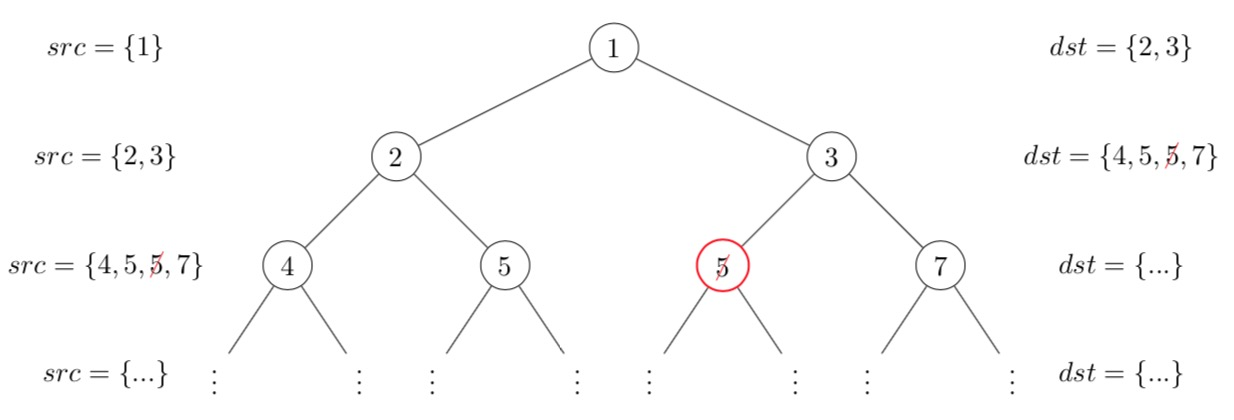
\includegraphics[width = \linewidth]{images/Distinct.jpg};
    \caption{SELECT DISTINCT}
\end{figure}
Hierbei liegt der Knoten 5 so, dass er in der 2. Rekursionsstufe 2 Mal in der Auswahl auftaucht. DISTINCT entfernt das Duplikat. Die Ergebnismenge, entfernt um die
Duplikate, wird als Input für die nächste Rekursionsstufe verwendet.
Die Ausgabe des verschachtelten SELECT Statement sind die Nachbarn der Knoten, der angegebenen Rekursionstiefe. Wird zum Beispiel ein
verschachteltes SELECT Statement der Tiefe 3 erstellt, so gibt dieses Statement alle Nachbarn 3. Grades ausgehend vom Startknoten an. Der Nachteil bei dieser Methode ist, dass
Zyklen in einem Graph nicht erkannt werden. Die Duplikatüberprüfung erfolgt nicht über mehrere Rekursionsstufen hinweg, sondern immer nur zwischen zwei Rekursionsstufen.

\subsection{Graphtraversierung mit Hilfe von rekursiven INNER JOIN}
Bei der Graphtraversierung mit Hilfe von rekursiven INNER JOIN soll der Graph traversiert werden, indem die Relationentabelle immer wieder mit sich selber verknüpft wird. Hierbei
wird das SQL Statement nicht automatisch generiert, sondern selbst geschrieben.
Die Ausgabe ist, ähnlich wie bei der Graphtraversierung mit Hilfe von verschachteltem SELECT Statement, die Nachbarn der Knoten, die sich auf der mitgegebenen Rekursionsstiefe
befinden. Ein Beispielstatement für den rekursiven INNER JOIN ist im Anhang gegeben (siehe \ref{JOIN}).

\subsection{Graphtraversierung mit Hilfe von selbstgeschriebenen Stored Procedure}
Bei der Graphtraversierung mit Hilfe von selbstgeschriebenen Stored Procedure wird der Graph mit Hilfe eines selbst erstellten Stored Procedure, das sich selber bis
zu einer mit gegebenen Rekursionstiefe wieder aufruft, traversiert (siehe \ref{recursiveFunction}). Die Abbruchbedingung wird dem Stored Procedure in Form einer Rekursionsstiefe mitgegeben. In jeder
Rekursionsstufe erstellt das Script 2 temporäre Tabelle. Eine temporäre Tabelle wird auf Basis eines Eingabeparameter erstellt. Diese temporäre Tabelle besitzt eine Spalte.
Diese Tabelle stellt die Spalte src der aktuellen Rekursionsstufe dar. Sie wird im IN Operator der WHERE Klausel verwendet um die 2. temporäre Tabelle zu erstellen. Die 2.
temporäre Tabelle beinhaltet die Spalte dst der aktuellen Rekursionsstufe.
%\lstsetsql

%\end{figure}
%\subsection{Beurteilung}